%% PNAStmpl.tex
%% Template file to use for PNAS articles prepared in LaTeX
%% Version: Apr 14, 2008


%%%%%%%%%%%%%%%%%%%%%%%%%%%%%%
%% BASIC CLASS FILE
%% PNAStwo for two column articles is called by default.
%% Uncomment PNASone for single column articles. One column class
%% and style files are available upon request from pnas@nas.edu.
%% (uncomment means get rid of the '%' in front of the command)

%\documentclass{pnasone}
\documentclass{pnastwo}

%%%%%%%%%%%%%%%%%%%%%%%%%%%%%%
%% Changing position of text on physical page:
%% Since not all printers position
%% the printed page in the same place on the physical page,
%% you can change the position yourself here, if you need to:

% \advance\voffset -.5in % Minus dimension will raise the printed page on the
                         %  physical page; positive dimension will lower it.

%% You may set the dimension to the size that you need.

%%%%%%%%%%%%%%%%%%%%%%%%%%%%%%
%% OPTIONAL GRAPHICS STYLE FILE

%% Requires graphics style file (graphicx.sty), used for inserting
%% .eps files into LaTeX articles.
%% Note that inclusion of .eps files is for your reference only;
%% when submitting to PNAS please submit figures separately.

%% Type into the square brackets the name of the driver program
%% that you are using. If you don't know, try dvips, which is the
%% most common PC driver, or textures for the Mac. These are the options:

% [dvips], [xdvi], [dvipdf], [dvipdfm], [dvipdfmx], [pdftex], [dvipsone],
% [dviwindo], [emtex], [dviwin], [pctexps], [pctexwin], [pctexhp], [pctex32],
% [truetex], [tcidvi], [vtex], [oztex], [textures], [xetex]

%\usepackage[dvips]{graphicx}

%%%%%%%%%%%%%%%%%%%%%%%%%%%%%%
%% OPTIONAL POSTSCRIPT FONT FILES

%% PostScript font files: You may need to edit the PNASoneF.sty
%% or PNAStwoF.sty file to make the font names match those on your system.
%% Alternatively, you can leave the font style file commands commented out
%% and typeset your article using the default Computer Modern
%% fonts (recommended). If accepted, your article will be typeset
%% at PNAS using PostScript fonts.

% Choose PNASoneF for one column; PNAStwoF for two column:
%\usepackage{PNASoneF}
\usepackage{PNAStwoF}

%%%%%%%%%%%%%%%%%%%%%%%%%%%%%%
%% ADDITIONAL OPTIONAL STYLE FILES

%% The AMS math files are commonly used to gain access to useful features
%% like extended math fonts and math commands.

\usepackage{amssymb,amsfonts,amsmath}

%\usepackage{subcaption}
\graphicspath{ {paper_figures2/} }

%\usepackage{sansmath}

%\usepackage[font={sf, small}]{caption}

%%%%%%%%%%%%%%%%%%%%%%%%%%%%%%
%% OPTIONAL MACRO FILES
%% Insert self-defined macros here.
%% \newcommand definitions are recommended; \def definitions are supported

%\newcommand{\mfrac}[2]{\frac{\displaystyle #1}{\displaystyle #2}}
%\def\s{\sigma}

\DeclareMathSizes{9}{8}{7}{7}

\DeclareMathOperator*{\argmin}{arg\,min}

\makeatletter
\newcommand{\customlabel}[2]{%
\protected@write \@auxout {}{\string \newlabel {#1}{{#2}{}}}}
\makeatother

%%%%%%%%%%%%%%%%%%%%%%%%%%%%%%
%% Don't type in anything in the following section:
%%%%%%%%%%%%
%% For PNAS Only:
\contributor{Submitted to Proceedings
of the National Academy of Sciences of the United States of America}
\url{www.pnas.org/cgi/doi/10.1073/pnas.0709640104}
\copyrightyear{2008}
\issuedate{Issue Date}
\volume{Volume}
\issuenumber{Issue Number}
%%%%%%%%%%%%

\begin{document}

%%%%%%%%%%%%%%%%%%%%%%%%%%%%%%


%% For titles, only capitalize the first letter
%% \title{Almost sharp fronts for the surface quasi-geostrophic equation}

\title{Temporal ordering and registration of cross-sectional imaging data}


%% Enter authors via the \author command.
%% Use \affil to define affiliations.
%% (Leave no spaces between author name and \affil command)

%% Note that the \thanks{} command has been disabled in favor of
%% a generic, reserved space for PNAS publication footnotes.

%% \author{<author name>
%% \affil{<number>}{<Institution>}} One number for each institution.
%% The same number should be used for authors that
%% are affiliated with the same institution, after the first time
%% only the number is needed, ie, \affil{number}{text}, \affil{number}{}
%% Then, before last author ...
%% \and
%% \author{<author name>
%% \affil{<number>}{}}

%% For example, assuming Garcia and Sonnery are both affiliated with
%% Universidad de Murcia:
%% \author{Roberta Graff\affil{1}{University of Cambridge, Cambridge,
%% United Kingdom},
%% Javier de Ruiz Garcia\affil{2}{Universidad de Murcia, Bioquimica y Biologia
%% Molecular, Murcia, Spain}, \and Franklin Sonnery\affil{2}{}}

\author{Carmeline~J.~Dsilva\affil{1}{Department of Chemical and Biological Engineering, Princeton University, Princeton, New Jersey, USA},
Bomyi~Lim\affil{1}{},
Thomas~J.~Levario\affil{2}{School of Chemical and Biomolecular Engineering, Georgia Institute of Technology, Atlanta, Georgia, USA},
Hang~Lu\affil{2}{},
Amit~Singer\affil{3}{Department of Mathematics, Princeton University, Princeton, New Jersey, USA} \affil{4}{Program in Applied and Computational Mathematics, Princeton University, Princeton, New Jersey, USA},
Stanislav~Y.~Shvartsman\affil{1}{} \affil{5}{Lewis-Sigler Institute for Integrative Genomics, Princeton University, Princeton, New Jersey, USA},
\and
Ioannis~G.~Kevrekidis\affil{1}{} \affil{4}{Program in Applied and Computational Mathematics, Princeton University, Princeton, New Jersey, USA}}

\contributor{Submitted to Proceedings of the National Academy of Sciences
of the United States of America}

%% The \maketitle command is necessary to build the title page.
\maketitle

%%%%%%%%%%%%%%%%%%%%%%%%%%%%%%%%%%%%%%%%%%%%%%%%%%%%%%%%%%%%%%%%
\begin{article}

\begin{abstract}
In studies of development, researchers are often presented with cross-sectional data, where each data point is a sample from a population fixed at a slightly different developmental time.
%
The goal is then to temporally order the data to reconstruct the developmental dynamics.
%
If each data point is a two-dimensional image, the images must first be registered before they can be temporally ordered.
%
When such data sets are large, noisy, and/or if the developmental changes are subtle, these tasks can be difficult to do by hand.
%
We present an automatic approach to register {\it and} temporally order cross-sectional data sets of images.
%
The mathematical techniques (angular synchronization for image registration, diffusion maps for temporal ordering, and
vector diffusion maps for simultaneously performing both tasks) are applicable to a wide variety of data sets and
require little {\it a priori} knowledge of the image features or the developmental dynamics.
%
We demonstrate the utility of our methods using a collection of images from a study of {\it Drosophila} embryogenesis.
\end{abstract}


%% When adding keywords, separate each term with a straight line: |
\keywords{temporal ordering | image registration}

%% Optional for entering abbreviations, separate the abbreviation from
%% its definition with a comma, separate each pair with a semicolon:
%% for example:
%% \abbreviations{SAM, self-assembled monolayer; OTS,
%% octadecyltrichlorosilane}

% \abbreviations{}

%% The first letter of the article should be drop cap: \dropcap{}
%\dropcap{I}n this article we study the evolution of ''almost-sharp'' fronts

%% Enter the text of your article beginning here and ending before
%% \begin{acknowledgements}
%% Section head commands for your reference:
%% \section{}
%% \subsection{}
%% \subsubsection{}

\dropcap{E}xperimental studies of developmental dynamics fall in two broadly defined categories: longitudinal and cross-sectional \cite{diggle2002analysis}.
%
In longitudinal studies, developmental progress is monitored over time for the same embryo.
%
In a cross-sectional study, one embryo contributes only a single snapshot of a chemical or morphological process along its developmental trajectory, and the developmental dynamics must be reconstructed from multiple snapshots of different embryos.
%
Both of these sampling schemes have their advantages and limitations, and both are extensively used by developmental biologists.
%
Here we focus on cross-sectional studies, which have a time-honored history and still present the only option for most organisms.
%
In a typical cross-sectional study, a group of developing embryos is fixed using a procedure that arrests their development and stained with chemicals that help visualize a handful of cellular processes.
%
Fixed embryos are then imaged using any given number of microscopy techniques.
%
Recent advances in large-scale physical manipulation and imaging of embryos have produced rapidly increasing volumes of cross-sectional data, in which every embryo is observed at a different geometric orientation and developmental time point.
%
Importantly, the ``age'' of any given embryo arrested in its development is not known to high accuracy.
%
In general, it is only known that a collection of embryos belongs to a certain time window.
%
In order to recover the developmental dynamics from such image datasets, snapshots of different embryos must be spatially aligned or registered to factor out the relevant symmetries (i.e., translations and rotations), and then ordered in time.
%
We present a general computational framework which greatly accelerates -and can combine- both of these tasks.

\begin{figure}[t]
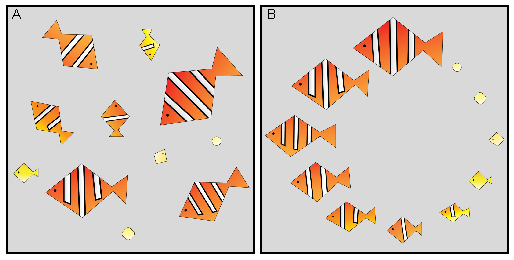
\includegraphics[width=8.4cm]{fig1}
\caption{{\it (A)} Fish, each in a different orientation and a different stage of development. {\it (B)} Fish, now rotationally registered and temporally ordered. For this caricature, the registration and ordering is easy to do ``by hand" because the data set is small and the developmental changes are easy to recognize.}
%\label{fig:fish}
\customlabel{fig:fish}{1}
\customlabel{subfig:fish_unordered}{\ref{fig:fish}{\it A}}
\customlabel{subfig:fish_ordered}{\ref{fig:fish}{\it B}}
\end{figure}
%
Temporal ordering and registration of images is straightforward when the number of images is small and differences between them are visually apparent.
%
As an example, Figure~\ref{fig:fish} shows a caricature of fish development, combining the processes of growth and color patterning.
%
In this case, temporal ordering can be accomplished by arranging the fish by size, which is monotonic with the developmental progress.
%
Image registration is based on obvious morphological landmarks, such as the position of head and fins.
%
On the other hand, real data poses nontrivial challenges, due to the number of images, measurement noise and variability, and the subtlety of the developmental changes.

To illustrate the issues associated with temporal ordering and registration of images, we use two data sets from an imaging study of signaling protein expression in the early fruit fly embryo, one of the leading model systems for studies of developmental dynamics.
%
The fruit fly embryo is shaped like a rice grain, approximately $1/2$~mm long.
%
By end of the $2^{nd}$ hour of development, sequential divisions of a fertilized egg generate a system where $\sim 6,000$ nuclei are uniformly arranged under the common plasma membrane.
%
During the $3^{rd}$ hour, the embryo undergoes the process of cellularization, whereby membranes that enclose nuclei into different cells grow in thickness (Figure~\ref{subfig:membranes}).
%
In conjunction with these morphological changes, concentration profiles of multiple regulatory molecules form inside the embryo, subdividing it into regions that give rise to future tissues and organs \cite{lim2013kinetics}.
%
During the $4^{th}$ hour of development, ...
%
Images in Figure~\ref{subfig:images_unordered} show optical sections at a fixed depth, perpendicular to the long axis of the embryo.
%
The embryos were fixed and stained with chemicals that help visualize nuclei (shown in gray) as well as the spatial distributions of two different proteins (shown in green and red) \cite{chung2010microfluidic}.
%
Each of the images reveals a uniform arrangement of nuclei and a nonuniform distribution of the two proteins, which are involved in patterning of the dorsoventral (back-to-belly) axis of the embryo.

Each image in Figure~\ref{subfig:images_unordered} comes from a different embryo, captured at a different rotation about the long axis and at a different and unknown point in time.
%
The goal is to register these images in a globally consistent way, and order them to be representative of the underlying developmental trajectory.
%
We will demonstrate that both of these tasks can be fully automated.

\begin{figure*}[t]
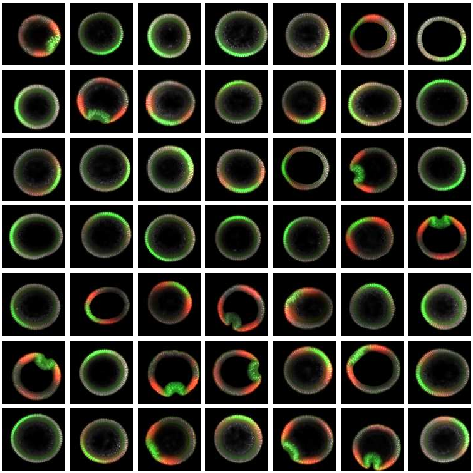
\includegraphics[width=6.5cm]{raw_data1}
\hfill
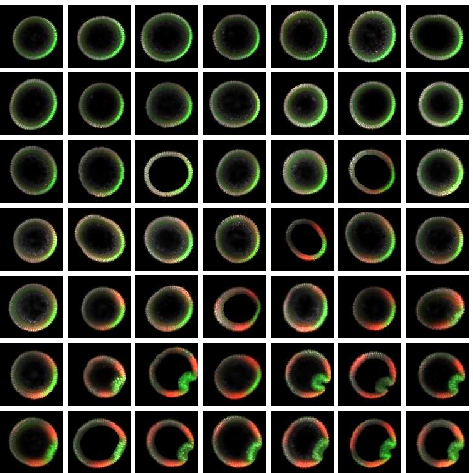
\includegraphics[width=6.5cm]{PCA_ordered}
\hfill
\begin{minipage}[b]{3.3cm}
\vspace{0in}
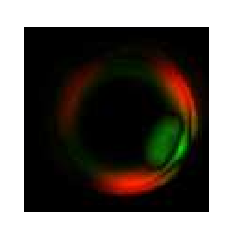
\includegraphics[width=3.3cm]{PCA_eigenimage1}
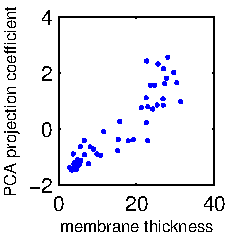
\includegraphics[width=3.3cm]{PCA_corr}
\end{minipage}
%\label{fig:fish}
\customlabel{fig:raw_data}{2}
\customlabel{subfig:raw_data1}{\ref{fig:fish}{\it A}}
\customlabel{subfig:raw_data2}{\ref{fig:fish}{\it B}}
\end{figure*}
%

\section{Results and Discussion}


\subsection{Image Registration}

Because each embryo is imaged in a different orientation, the first task is to align or {\em register} the images so that they are in a consistent frame of reference.
%
We use angular synchronization to register our images. 
%
This technique is very general, as it requires no template image or feature points. 
%
Furthermore, it has been shown to be robust to noise.
%
Implementation details are given in the {\it SI appendix}. 

Figure ... shows the images from Figure ..., registered using angular synchronization.
%
The important features that our eye can visually detect (e.g., the green Dorsal peaks) have been aligned, even though the algorithm does not require identification of such features.

\subsection{Temporal Ordering using Principal Component Analysis}

We will use dimensionality reduction techniques to temporally order our data.
%
Although our images are inherently high-dimensional (number of pixels $\times$ number of channels), we assume that they lie on a low-dimensional curve, and that this curve is parameterized by time.
%


For the images shown in Figure ...., the dynamics are relatively simple, and we can use principal component analysis (PCA) to order the images.
%
PCA extracts a set of {\it eigenimages} from the data, such that each data point can be (approximately) described as a linear combination of these eigenimages. 
%
In our dataset, each data point can be effectively described by a multiple of a single eigenimage, i.e., the images lie on a line in a very high-dimensional space.
%
We can therefore sort these images along this line to temporally order them in time.


Figure ... shows the images, now ordered using PCA. 
%
The first eigenimage is also shown.

In this simple example, we can validate our ordering using an independent time marker.
%
Figure ... shows the rank correlation betrween the two orderings.
%
Rank correlation is 0.9199.

Although PCA can successfully order the data set shown in Figure ..., it can only do so because the data lie on in a one-dimensional, {\em linear} subspace.
%
In general, the developmental trajectory is not guaranteed to be linear. 
%
This can be seen in the late images of Figure ... that the ordering is not entirely correct.
%
We can also see this from the projection onto the first two eigenimages, shown in Figure ...
%
The data clearly lie on a one-dimensional curve, but the curve is nonlinear at late times. 
%
This motivates us to use nonlinear dimensioanlity reduction techniques to temporally order our data.

\subsection{Temporal Ordering Using Diffusion Maps}
We will use diffusion maps, a technique which is robust to noise and broadly applicable to a wide variety of data types.
%

We can use diffusion maps to analyze more complex data sets where the dynamics are clearly nonlinear.
%
Figure ... shows a data set from the $4^{th}$ hour of development.
%
The dynamics are significantly more complex. 
%
However, we can still use diffusion maps to temporally order the data.

We have no time marker with which to validate our orderings in this time period. 
%
However, there are noticable features in the ordering that we can see are consistent with peviously known dynamics. 
%
For example, ....

\begin{figure*}[t]
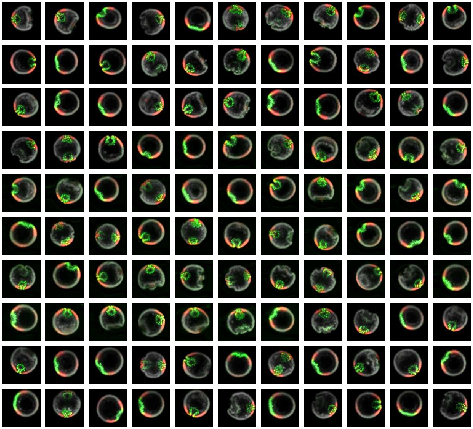
\includegraphics[width=8.4cm]{raw_data2}
\hfill
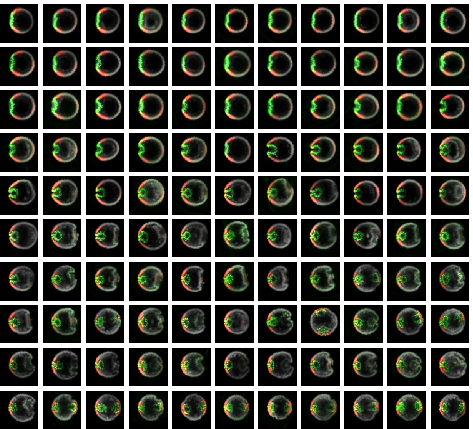
\includegraphics[width=8.4cm]{VDM_ordered} \\
\centering
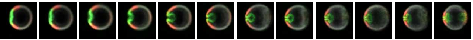
\includegraphics[width=16.8cm]{average_trajectory}
%\label{fig:fish}
\customlabel{fig:raw_data}{2}
\customlabel{subfig:raw_data1}{\ref{fig:fish}{\it A}}
\customlabel{subfig:raw_data2}{\ref{fig:fish}{\it B}}
\end{figure*}


\section{Conclusions}

\end{article}

\end{document}

